\documentclass[../../main.tex]{subfiles}
\begin{document}

\chapter{CostCompiler}
CostCompiler é un interprete per il linguaggio di programmazione definito nel capitolo precedente Grammatica \ref{sec:grammatica}. Una volta ricevuto il programma, CostCompiler procede alla verifica e correttezza sintattica e semantica del programma, successivamente si occupa della generazione dell'albero di sintassi astratta. 
Questo albero rappresenta una versione astratta del programma, che astrae i dettagli sintattici del codice e si concentra sulla sua struttura logica, associando ad ogni costrutto (eg.\textit{if-then-else} un unico nodo, \textit{IfNode} presente nel omonimo file in src/ast) i rispettivi sottonodi(nel caso di \textit{IfNode} conterrá la guardia condizionale e i due statement).
Dopo aver generato l'albero di sintassi astratta,CostCompiler si occupa della verifica Semantica \ref{sec:semantica} del linguaggio andando ad effettuare i controlli semantici e di tipo sul programma in input, andando a garantire alcune invarianti (eq. Le chiamate di funzioni devono rispettare i tipi di ritorno).\\
Una volta effettuata la verifica semantica, CostCompiler procede con la generazione delle equazioni di costo, andando a visitare l'AST secondo determinati criteri, ad ogni nodo figlio verrá passata una Mappa che contiene la mappatura di ogni variabile in una stringa che sará la stessa stringa che compare nelle equazioni di costo.\\
Ogni nodo figlio invocato attraverso la funzione \textit{toEquation()} ritorna una stringa, rappresentante l'equazione di costo del nodo figlio, e il padre va a concatenare le stringhe dei figli(anche in base al tipo di figlio da cui ricevere l'equazione), ad esempio la \textit{return $<$EXP$>$ } sará diverso dal \textit{return }$<$function$(Par)>$.\\
Il risultato finale di questo processo di concatenazione attraverso determinati nodi dell'AST é la generazione delle equazioni di costo. 
Una volta generate le equazioni di costo, CostCompiler le stampa in un file \textit{equation.txt} inoltre lancia il risolutore PUBS \ref{sec:pubs} che va a calcolare gli upper bound del programma da stampare a video.
Riportiamo un esempio di equazione di costo generata da CostCompiler dato un programma scritto in HLCostLang:
    \begin{lstlisting}[language=Java, caption={Listing8}]
    struct Params {
        address: array[int],
        payload: any,
        sender: string
    }
    service PremiumService : (string) -> void;
    service BasicService : (any) -> void;
    (isPremiumUser: bool, par: any) => {
        if ( isPremiumUser ) {
            call PremiumService("test");
        } else {
            call BasicService( par);
        }
    }
\end{lstlisting}
Una volta preso in input Listing8, CostCompiler genera le seguenti equazioni di costo:
\begin{lstlisting}[language=Java, caption={Equazioni di costo per Listing8}]
eq(main(P,ISPREMIUMUSER0,B),0,[if9(ISPREMIUMUSER0,P,B)],[]).
eq(if9(ISPREMIUMUSER0,P,B),nat(P),[],[ISPREMIUMUSER0=1]).
eq(if9(ISPREMIUMUSER0,P,B),nat(B),[],[ISPREMIUMUSER0=0]).
\end{lstlisting}
Andando a descriverle ci troveremo ad avere una equazione per la regola \textit{init}, dove vediamo che \textit{main} viene chiamata con costo 0 e verrá chiamata \textit{if9} con parametri \textit{ISPREMIUMUSER0,P,B}.\\
$P$ e $B$ sono il costo costante delle chiamate ai servizi \textit{isPremiumUser} e \textit{BasicService}, mentre \textit{ISPREMIUMUSER0} sará la valutazione del parametro \textit{isPremiumUser} che sará 1 se vero, 0 altrimenti; in altri termini \textit{ISPREMIUMUSER0} sará la valutazione della guardia del costrutto \textit{if-then-else} e verrá eseguita la chiamata al servizio \textit{PremiumService} se \textit{ISPREMIUMUSER0} sará 1 con costo $nat(P)$, altrimenti verrá eseguita la chiamata al servizio \textit{BasicService} con costo $nat(B)$. 
Una volta avere generato l'equazioni di costo dal programma, lo stampiamo in un file \textit{equation.txt}, cosi da poter eseguire PUBS(A Practical Upper Bounds Solver), per determinarci l'Upper Bound del programma.
L'obiettivo di PUBS(come vedremo in seguito \ref{sec:pubs}) é quello di ottenere automaticamente upper bound in forma chiusa per i sistemi di equazioni di costo, di conseguenza calcola i limiti superiori per la relazione di costo indicata come "Entry", oltre che per tutte le altre relazioni di costo di cui tale "Entry" dipende.

\section{Regole di Inferenza}
\label{sec:inference_rule}
I programmi di costo sono elenchi di equazioni che hanno termini:
$$f(\overline{x} ) = e + \sum_{i \in 0..n} f_i (\overline{e_i}) \quad \quad \quad \quad[\varphi ]$$
Dove le variabili si presentano nel lato destro e in $\varphi $ sono un sottoinsieme di $\overline{x}$; mentre $f$ e $f_i$ sono i simboli delle funzioni.
Ogni funzione ha un right-hand-side che é un'espressione aritmetica che può contenere:
\begin{itemize}
    \item Un'espressione in Presburger aritmetica (PA):
    $$e ::= x \quad | \quad q \quad | \quad e + e \quad | \quad e - e \quad | \quad q \cdot e \quad |  max(e_1,\dots,e_n)$$
    Dove $x$ é una variabile, $q$ é una costante intera, $e_1,\dots,e_n$ sono espressioni aritmetiche e $max$ é un operatore che restituisce il massimo valore tra le sue espressioni.
    \item Un numero di invocazioni di funzioni di costo: $f_i (\overline{e_i})$.
    \item La guardia $varphi$ é un vincolo congiuntivo lineare nella forma: $e_1 \geq e_2$ dove $e_1$ e $e_2$ sono espressioni aritmetiche di Presburger.
\end{itemize} 

La soluzione di un equazione di costo é il calcolo dei limiti di un particolare simbolo di una funziona(generalmente la prima equazione) e i limiti sono parametrici nei parametri formali dei simboli della funzione.
Definiamo un insieme di regole di inferenza che raccolgano frammenti di programmi di costo che vengono poi combinati in modo diretto dalla sintassi.
Usiamo una variabile di ambiente $ \varGamma $ come dizionari:
\begin{itemize}
    \item $\varGamma$ prende un servizio o un parametro e ritorna un espressione aritmetica di Presburger che di solito é una variabile.
    \item Quando scriviamo $\varGamma + i : \quad Nat $, assumiamo che i non appartenga al dominio di $\varGamma$.
\end{itemize}
I giudizi hanno forma:
\begin{itemize}
    \item $\varGamma \vdash e : Nat$ che significa che il valore di E in $e$ é rappresentato dalla costEspression $E$
    \item $\varGamma \vdash S : e ; C; Q $ significa che il costo di S nell'ambiente $\varGamma$ é $e + C$ dato un insieme di equazioni Q
\end{itemize}


\begin{align}
    &\mathrule{main}{
        \begin{aligned} \varGamma \vdash S : e ; C; Q  \quad \quad
        \overline{w} = \text{Var}(\overline{p},e) \cup \text{Var(C)}
        \end{aligned}
        }{\varGamma \vdash \overline{p}  \rightarrow \{S\}: 0 ;\emptyset;Q';C} \\
    &\mathrule{call}{\varGamma \vdash S : e ; C; Q}{\varGamma \vdash \text{call h}(\overline{E}) S : e + e' ; C; Q}\\
    &\mathrule{if}{
    \begin{aligned}
        &\varGamma \vdash E : \varphi  \quad \quad \varGamma \vdash S : e'; C; Q \quad \varGamma \vdash S : e"; C'; Q'\\
        &W = Var(e, e', e") \cup Var(C) \quad \quad \quad Q" =\big[ \begin{aligned}
            &\text{if}_l(\overline{w})  = e'+c[\varphi]\\
            &\text{if}_l(\overline{w})  = e"+c[\neg \varphi]\\
        \end{aligned}\big] \\
    \end{aligned}    
    }{\varGamma \vdash \text{if } E \text{ then } S_1 \text{ else } S_2 : 0; if_l(\overline{w}); Q; Q'; Q"}\\
    &\mathrule{let}{\varGamma + i : Not \quad \quad \quad \quad \overline{w} = Var(E) \cup Var(c)}{\varGamma \vdash \text{let } i = e \text{ in } S : S;e ; C; Q}\\
    &\mathrule{for}{
        \begin{aligned}
            &\varGamma \vdash M: e \quad \quad \quad \quad \varGamma \vdash i : Not\quad \quad \quad \quad \varGamma \vdash S : e'; C; Q\\
            &\overline{w} = Var(e, e') \cup Var(C) \ i \quad \quad \quad \quad Q' = \big[ \begin{aligned}
                &\text{for}_l(i,\overline{w}) = e + c\quad [i \lq e]\\
                &\text{for}_l(i,\overline{w}) = 0 \quad \quad [i \geq e]\\
            \end{aligned}\big]
        \end{aligned}
    }{\varGamma \vdash \text{for i in (0,M) } \text{ { S } } : 0; for_l(0,\overline{w}); Q; Q'}\\
\end{align}

Riassumiamo le regole descritte in precedenza:\\
\begin{itemize}
    \item Regola$[$call$]$ gestisce l'invocazione di un servizio; il costo della call sará il costo di $S$ piú il costo per l'accesso al servizio $h$ 
    \item Regola$[$if$]$ gestisce il costrutto condizionale;quando la guardi é un'espressione definita in aritmetica di Presburger e il costo verrá rappresentato da entrambi i rami con i due condizionali $\varphi $ e $\not \varphi$.\\Rappresentiamo a livello di equazione $if_l$ dove $l$ é la linea di codice dové inizia il costrutto.
    \item Regola $[$for$]$ descritto all'interno del rispettivo frammento di codice come $for_l$ per lo stesso motivo citato in precedenza; Definiamo i come Nat e verifichiamo che non sia presente nell'ambiente $\varGamma$ e scriviamo il rispettivo $S$ come caso base in cui $e \geq i$ oppure $i \geq e + 1$
    \item Regola $[$LetIn$]$ Dove viene definita E nell'ambiente $\varGamma$ con costo e(il costo per eseguire l'espressione $e$). Andremo a valutare se in $\varGamma$ é presente $E$ e andiamo a valutare $\varGamma \vdash S$ che ritornerá un'equazione $Q'$ con costo $C$.
\end{itemize}
\section{Generazione delle Equazioni di costo}

La generazione delle equazioni di costo viene eseguita andando a implementare le regole di inferenza viste in precedenza.
Ogni nodo all'interno del nostro AST contiene il metodo \textit{toEquation()} che prende come argomento la variabile del nostro ambiente $\varGamma$ e sará appunto un dizionario.
Questo dizionario di tipo $EnvVar$ é un HashMap che contiene come chiave l'oggetto Nodo della variabile e come valore la stringa rappresentante.
Abbiamo deciso di utilizzare questo approccio per focalizzarci sull'efficienza del farci restituire la variabile che mappa quel determinato Nodo, senza dover andare a cercare all'interno dell'HashMap la chiave che mappa quel valore, cosa che viene fatta all'inserimento di un Nodo.
L'inserimento del nodo peró non sempre é un operazione onerosa per il fatto che abbiamo gia il controllo semantico che ci garantisce che non ci saranno variabili non dichiarate oppure variabili non dichiarate prima del loro utilizzo.\\
Andiamo ad analizzare un esempio semplice, all'interno del Nodo di tipo \textit{CallService.java} che rappresenta l'invocazione di un servizio: abbiamo il metodo \textit{toEquation()} che prende come argomento l'ambiente $\varGamma$ e restituisce una stringa che rappresenta l'equazione di costo del nodo. Questa sottostringa sará poi riportata all'interno dell'equazione di costo del nodo padre.

\begin{lstlisting}[language=Java]
    @Override
    public String toEquation(EnvVar e) {
        return "nat("+e.get(this)+")" + (stm!= null ? "+"+stm.toEquation(e) : "");

    }
\end{lstlisting}

La funzione $e.get(this)$ ritorna la variabile mappata per quel determinato nodo, ritorna quindi una stringa che rappresenta la variabile all'interno dell'equazione di costo. La funzione $stm.toEquation(e)$ é la chiamata sul metodo \textit{toEquation()} del nodo figlio, che restituirá la stringa rappresentante l'equazione di costo del nodo, andando a richiamare il medesimo metodo sui sottonodi contenuti all'interno del nodo figlio, e così via.\\
Per avere una panoramica completa del processo di generazione delle equazioni di costo, riportiamo il frammento di codice della funzione $toEquation()$ del $programNode$, che rappresenta il nodo principale del nostro AST, che andrá a richiamare il metodo $toEquation()$ su tutti i nodi figli e andrá a concatenare le stringhe risultanti al fine di generare l'equazione finale.
\begin{lstlisting}[language=Java, caption={toEquation() del ProgramNode}]
    public String toEquation(EnvVar e){

        for (Node n : decServices){
            n.checkVarEQ(e);
        }
        StringBuilder equ = new StringBuilder();
        for(Node n : funDec){
            equ.append(n.toEquation(e));
        }
        equ.append(main.toEquation(e));
        return equ.toString();
    }
\end{lstlisting}

Come possiamo vedere, prima di generare le equazioni di costo del programma, andiamo a controllare che le variabili dichiarate all'interno dei servizi siano presenti all'interno dell'ambiente $\varGamma$ e le mappiamo con determinate stringhe che appariranno nelle equazioni. Successivamente andiamo a iterativamente all'interno delle singole funzioni le generiamo e le concateniamo alla stringa che rappresenta le equazioni di costo del programma.\\
Infine ci occupiamo di generare le equazioni di costo della funzione main, che saranno concatenate anch'esse con la stringa che rappresenta le equazioni di costo del programma.

\section{PUBS}
\label{sec:pubs}
PUBS (Pratical Upper Bounds Solver) ha l'obiettivo di ottenere automaticamente un'upper bound in forma chiusa per i sistemi di equazioni di costo, di conseguenza calcola i limiti superiori per la relazione di costo indicata come "Entry".

\subsection{Analisi di costo}
CCome analisi statica dei costi, miriamo a ottenere risultati analitici per un dato programma $P$, i quali consentano di vincolare il costo dell'esecuzione di $P$ su qualsiasi input $x$, senza dover effettivamente eseguire $P(x)$.\autocite{albert2011closed}\\
Partiamo da un esempio, che ci aiuterá a capire meglio il concetto di analisi di costo, partendo da un programma java:
\begin{lstlisting}[language=Java, caption={Esempio di Analisi di Costo}, label={lst:costAnalysisExample}]
    public void m(int[ ] v) {
        int i=0;
        for (i=0; i<v.length; i++)
        if (v[i]%2==0) m1();
        else m2();
    }
\end{lstlisting}
Le seguenti relazioni catturano il costo di esecuzione di questo programma:
\begin{figure}[H]
    \centering
    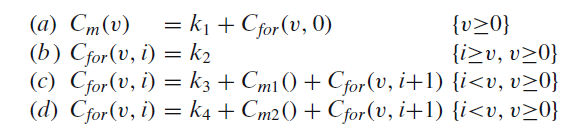
\includegraphics[width=0.6\textwidth]{basicExample.png}
    \caption[short]{Relazioni di costo del programma \ref{lst:costAnalysisExample}}
\end{figure}
%%Continua

Un esempio già più completo si trovo nel paper \textit{Automatic Inference of Upper Bounds for Recurrence Relations in Cost Analysis} \autocite{albert2008automatic}:
\begin{figure}[H]
    \centering
    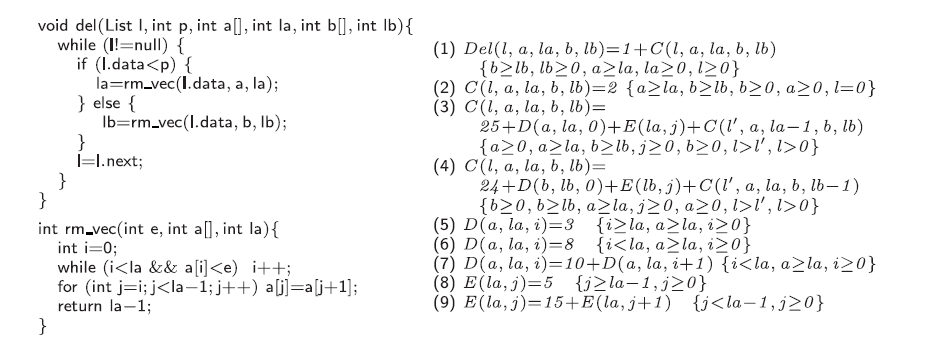
\includegraphics[width=0.9\textwidth]{costAnalysisExample.png}
    \caption{Esempio di Analisi di Costo}
    \label{fig:costAnalysisExample}
\end{figure}
Come possiamo vedere dall'immagine sopra, abbiamo a sinistra un programma scritto in java mentre a destra abbiamo l'analisi di costo del programma.\\
Il metodo $del$ prende in input una lista $l$, un pivot $p$, due array ordinati di interi $a$ e $b$ e $la$ e $lb$ che indicano rispettivamente le posizione occupate in $a$ e $b$.
Inoltre, si prevede che l'array $a$ contiene gli elementi inferiori al pivot $p$, mentre $b$ rispettivamente ne conterrá i valori maggiori o uguali.
Partiamo dal presupposto che tutti i valori in $l$ siano contenuti in $a$ o $b$, e il metodo $del$ rimouve tutti i valori in $l$ da $a$ o $b$ rispettivamente.
Il metodo $rm_vec$ rimouve un dato valore $e$ da un array $a$ di lunghezza $la$ e ne ritorna la nuova lunghezza.\\
Gli autori del paper \autocite{albert2008automatic},applicano l'analisi dei costi a questo programma, approssimando il costo del metodo $del$ in termini di istruzione bytecode eseguite.\\
La figura \ref{fig:costAnalysisExample} presenta i risultati dell'analisi, dopo aver effettuato una valutazione parziale.
Nei risultati dell'analisi le strutture dati dell'analisi vengono astratte in base alle loro dimensioni:$l$ rappresenta la lunghezza massima del percorso della corrispondente struttura dinamica, $a$ e $b$ sono le lunghezze degli array corrispondenti, mentre $la$ e $lb$ sono i valori interi delle variabili.
Ci sono nove equazioni che definiscono la relazione $ del $ che corrisponde al costo del metodo $del$ e 3 relazioni ricorsive ausiliarie C, D, E; ciascuna delle quale corrisponde a un ciclo:(C: Ciclo while in $del$, D: ciclo while in $rm_vec$ e E: Ciclo for in $rm_vec$).
Ogni equazioni é definita con una serie di vincoli che catturano le relazioni dimensionali tra i valori delle variabili della parte sinistra(lhs) e della parte destra(rhs).
Prendiamo in esempio le equazioni per $D$ Eq5. e Eq.6 rappresentano casi base per l'uscita dal ciclo ovvero quando $i \geq la$ e $a[i]\geq e$.
Per le nostre misurazioi di costo, vengono contati 3 istruzioni bytecode in Eq.5 e 8 in Eq.6.
Il costo per eseguire un iterazione del ciclo é rappresentato da Eq.7, dove la condizione $i < la$ deve essere soddisfatta e la variabili $i$ è incrementata di uno ad ogni chiamata ricorsiva.

\subsection{Relazione di Costo} 
Un'espressione di costo di base é un'espressione simbolica che indica le risorse accumulate e i blocchi fondamentali non ricorsivi per la definizione delle \textit{relazioni di costo}.
\newtheorem{definition}{Definizione}
\begin{definition}(Espressione di costo di base)\\
Le espressioni di costo sono della forma $$exp :: = a | nat(l) | exp + exp | exp * exp |exp^a |log _a (exp) | max(s) | \frac{exp}{a} | exp - a   $$
dove $a \geq 1$, $l$ é un'espressione lineare, $S$ é un insieme non vuoto di espressioni di costo, $nat : \mathbb{Z}  \rightarrow \mathbb{Q} ^+$ é definita come $nat(v) = max({v,0})$ e $exp$ soddisfa per qualsiasi assegnamento di $\overline{v}$ per vars($exp$) si ha $exp[ vars(\frac{exp}{\overline{v}})]$
\end{definition}

Le espressioni di costo di base godono di due proprietá:
\begin{itemize}
    \item Sono sempre valutate per valori non negativi
    \item Rimpiazzando una sottoespressione $nat(l)$ con $nat(l')$ tale che $l \geq l'$ , il risultato é un upper bound per l'espressione originale.
\end{itemize}
L'analisi dei costi di un programma produce multiple relazioni interconnesse, generando un \textit{sistema di relazioni di costo}(CRS)

\begin{definition}(Sistema di relazioni di costo)\\
    Un sistema di relazioni di costo S é un set di equazioni della forma $\langle C(\overline{x}) = exp + \sum_{i = 0}^n D_i(\overline{y_i}), \varphi \rangle$  dove $C$ e $D_{0,\dots, i}$ sono relazioni di costo; tutte le variabili in $\overline{x}$ e $\overline{y_i}$ sono variabili distinte, e $\varphi$ é una relazione di dimensione tra  $\overline{x} \cup vars(exp) \cup \overline{y_i}$.
\end{definition}

Dato $S$ sistema di relazioni di costo, $rel(S)$ indica l'insieme delle relazioni di costo definite in S, $def(S,C)$ indica il sottoinsieme di equazioni in S il cui lato sinistro é della forma $C(\overline{x})$.
Possiamo supporre che tutte le equazioni definite in $def(S,C)$ abbiano variabili con lo stesso nome nella parte sinistra.
Inoltre si suppone che ogni relazione di costo che appare nella parte sinistra dell'equazione $S$ deve essere in $rel(S)$.
\subsubsection{Semantica per CRS}
Data una CRS $S$, una call é della forma $C(\overline{v})$ dove $C \in rel(S)$ e $\overline{v}$ sono valori interi.
Le \textit{call} sono valutate in due fasi, in cui la prima permette la costruzione un albero di evoluzione, mentre la seconda ottiene un valore di $\mathbb{R}^+$ da aggiungere alla costante che appare nell'albero di valutazione.
Gli alberi di evoluzione sono costruiti espandendo iterativamente i nodi che includono chiamate alle relazioni. Ogni espansione avviene rispetto a un'istanza appropriata della parte destra di un'equazione applicabile. Se tutte le foglie dell'albero contengono un'espressione di costo di base, allora non ci sono più nodi da espandere e il processo termina. Questi alberi sono rappresentati utilizzando termini annidati, del tipo node(Call; Local\_Cost; Children), in cui Local\_Cost è una costante in $\mathbb{R}^+$ e Children è una sequenza di alberi di evoluzione.

\begin{definition}(\textbf{Albero di evoluzione})
    Data una CRS $S$, una call $C(\overline{v})$, un albero node $(C(\overline{v}); e; \overline{t})$ é un albero di evoluzione per $C(\overline{v})$ in S, indicato con $Tree (C(\overline{v},S))$, se:
    \begin{enumerate}
        \item c'é una denominazione parziale dell'equazione $\langle C(\overline{x}) = exp + \sum_{i = 0}^k D_i(\overline{y_i}), \varphi \rangle$
        \item esiste un assegnamento di valori interi $\overline{w}$ a $\overline{v_i}$ per $var(exp), \overline{y_i}$ rispettivamente tali che $\varphi[vars(exp)/\overline{w}, \overline{y_i}/\overline{v_i}]$ é soddisfacibile in $\mathbb{Z}$
        \item $e = exp[vars(exp)/\overline{w}]$, $T_i$ é un albero di evoluzione  $tree(D_i (\overline{v_i}, S))$ with $i \in 0,\dots,k$ 
    \end{enumerate}
\end{definition}

Nel processo di risoluzione di $C(\overline{v})$ ci possono essere diverse equazioni applicabili, e quindi diversi alberi di evoluzione.
Al passo 2 si cerca un assegnamento per le variabili nella parte destra di $\epsilon$. Al passo 3 gli assegnamenti sono applicati ad exp e si continua ricorsivamente valutando le call.
$Tree(C(\overline{v}, S))$ viene usato per denotare l'insieme di tutti gli alberi di evoluzione per $C(\overline{v})$.
\subsection{Stima del costo per Nodo}
Tutte le espressioni nei nodi sono istanze delle espressioni che compaiono nelle equazioni corrispondenti. Pertanto, il calcolo di $costr^+(\overline{x})$ e $costnr^+(\overline{x})$ può essere effettuato trovando innanzitutto un limite superiore di tali espressioni e quindi combinandoli attraverso un operatore di massimo. Prima calcoliamo gli invarianti per i valori che le variabili delle espressioni possono assumere rispetto ai valori iniziali e li utilizziamo per derivare limiti superiori per tali espressioni.\\
Calcolare le invarianti(in termini di vincoli lineari), in modo che raggruppa tutte le chiamate ai contesti di una relazione $C$, tra gli argomenti di una chiamata iniziale e ogni chiamata durante la valutazione che può essere fatta usando $Loops(C)$
Ovvero, se é presente un vincolo lineare $\psi$ tra gli argomenti di una chiamata iniziale $C(\overline{x_0})$, quelli di una chiamata ricorsiva $C(\overline{x})$, indicato con $\langle C(\overline{x_0})\rightsquigarrow  (\overline{x}, \psi)\rangle$, e se esiste il ciclo $C(\overline{x_0}) \rightsquigarrow (\overline{y},\varphi)\in Loops(C)$ allora é possibile applicare il ciclo a uno o piú step e prende un nuovo calling context $\langle C(\overline{x_0})  \rightsquigarrow (\overline{y}), \overline{\exists} \cup \overline{y_i}\dot \psi \land \varphi\rangle$
Una volta che le invarianti sono state stabilite, è possibile determinare il limite superiore delle equazioni di costo massimizzando la loro parte nat indipendentemente. Questo approccio è reso possibile grazie alla proprietà di monotonia delle espressioni di costo. Considerando un'equazione di costo nella forma $\langle  C(\overline{x}) = exp + \sum_{i=0}^k C(\overline{y_i}), \varphi \rangle$ e un invariante $C(\overline{x_0})\rightsquigarrow C(\overline{x}, \varPsi) $ ,una funzione può calcolare un limite superiore $f'$ per ogni $f$ che compare nell'operatore $nat$. Tale funzione sostituisce $f$ con un limite superiore nelle espressioni $exp$ in cui non è possibile determinare un limite superiore e la funzione tornerà $\infty$. Se questa funzione è completa, ovvero se i $\varPsi$ e $\varphi$implicano che esiste un limite superiore per un dato $nat(f)$, allora possiamo trovare un limite superiore su $\varPsi '$.\\
\autocite{amslaurea3135}

\subsection{PUBS in pratica}
Prendiamo in considerazione il seguente esempio di programma dato in input a CostCompiler:
\begin{lstlisting}[caption={Listing 1}]
struct Params {
	address: array[int],
	payload: any,
	sender: string
}
service PremiumService : (string) -> void;
service BasicService : (any) -> void;
(isPremiumUser: bool, par: any) => {
	if ( isPremiumUser ) {
		call PremiumService("pippo");
	} else {
		call BasicService( par);
	}
}
\end{lstlisting}

PUBS (Pratical Upper Bounds Solver) ha l'obiettivo di ottenere automaticamente un'upper bound in forma chiusa per i sistemi di equazioni di costo, calcola i limiti superiori per la relazione di costo indicata come "Entry", oltre che per tutte le altre relazioni di costo di cui tale "Entry" dipende.
Nell'output di PUBS vengono mostrati anche i passaggi intermedi eseguiti che coinvolgono il calcolo delle funzioni di classificazione e degli invarianti di ciclo.

\begin{figure}[H]
    \centering
    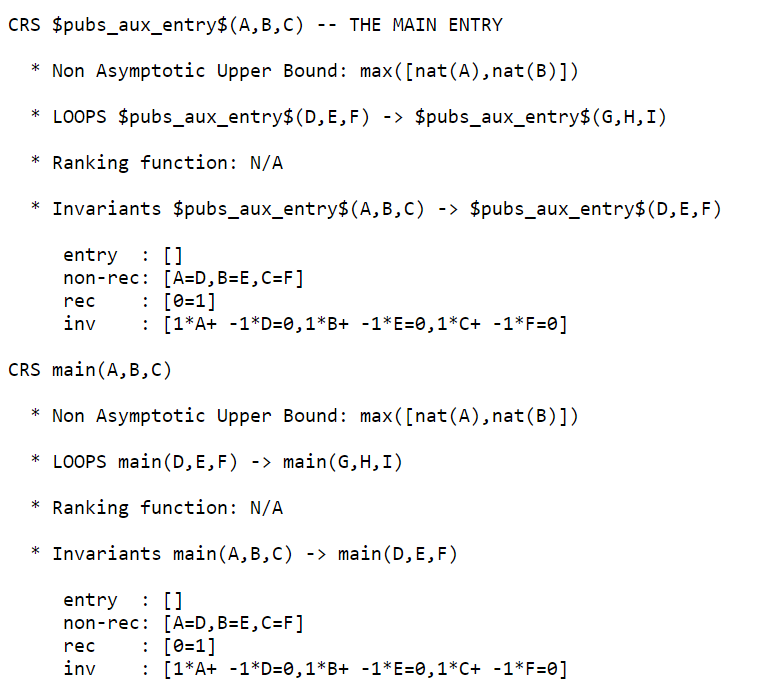
\includegraphics[width=0.9\textwidth]{pubs_example.png}
    \caption{Esempio di output PUBS su Listing 1}
\end{figure}
Come vediamo nell'immagine sopra, PUBS restituisce un analisi dell'intera equazione ($pub\_aux\_entry$) e delle singole funzioni da cui essa dipende, in questo caso $pubs\_aux\_if9$ e $pubs\_aux\_main$.
In questo caso con ``Listing1'' abbiamo un Upper Bound non Asintotico di $max(Nat(A), Nat(B))$ che ci determina che il costo del programma dipende dalle variabili A e B, e che il costo del programma sará il massimo tra i due.
PUBS ha una grammatica che definisce l'equazione di costo che deve essere rispettata da ogni equazione di costo generata da CostCompiler, che é la seguente:
\begin{lstlisting}[language=ANTLR, caption={Grammatica PUBS}]
<equation> ::= eq(Head,costExpression,[listOfCall],[ListOfSizeRelation]).

<Head> ::= Name | Name(Par).

<costExpression> ::= nat(<variable>) 
            | <costExpression> + <costExpression> 
            | <costExpression> - <costExpression> 
            | <costExpression> * <costExpression> 
            | max(<costExpression>,<costExpression>).
                
<listOfCall> ::= [] | <call> <listOfCall>.
<call> ::= <function>(<listOfParameters>).
<listOfParameters> ::= [] | <variable> <listOfParameters>.
\end{lstlisting}
Dove $<$Head$>$ é il nome della entry che andremo ad analizzare insieme ai suoi parametri.
CostExpression é l'espressione di costo che rappresenta il costo della entry e rispetta la grammatica della aritmetica di Presburger.
ListOfCall é la lista delle chiamate alle altre entry, che sono rappresentate come $<$call$>$ e $<$listOfCall$>$, la lista di queste chiamate; in questo modo PUBS riesce a costruire un grafo delle dipendenze tra le entry.
Infine abbiamo $<$listOfSizeRelation$>$ che sará la lista delle relazioni di costo che dipendono dalla entry che stiamo analizzando, e che PUBS andrá a calcolare.
Riportiamo un'altro esempio di equazione di costo generata da CostCompiler, questa volta per il programma scritto in Listing6:
\begin{lstlisting}[caption={Listing 6}, language=Java]
    service BasicService: (int) -> void;
    fn svc(i: int) -> void{
        for(m in (0,10)){
            call BasicService(i)
        }
    }
    (len : int) => {
        svc(len)
    }
\end{lstlisting}
Come vediamo, la funzione $init$ chiamerá la funzione $svc$ con parametro len, che a sua volta chiamerá la funzione BasicService per 10 volte, quindi il costo del programma sará l'invocazione della funzione $svc + 10 \cdot nat(B)$, dove $nat(B)$ é l'invocazione del servizio \textit{BasicService}.\\
L'equazione di costo risultante sará la seguente:
\begin{lstlisting}[language=Java,caption={Equazione di costo PUBS per Listing6}]
    eq(main(B),1,[svc(B)],[]).
    eq(svc(B),0,[for3(0, B)],[] ).
    eq(for3(M, B) ,nat(B),[for3(M+1, B)], [10>= M]).
    eq(for3(M, B) ,0,[],[M >= 10+ 1]).
\end{lstlisting}

Nella prima riga troviamo l'entry $main$ che prende in input B, con costo 1, chiama la funzione $svc$.
Quest'ultima andrá a chiamare la funzione $for3$ inserendo un'ulteriore parametro che sará il counter del ciclo con parametro 0 e B, che avrá costo 0 in caso $M >= 10 + 1$ altrimenti avrá costo $nat(B)$.
E come controprova mostriamo ora il risultato di PUBS su Listing6:
\begin{figure}[H]
    \centering
    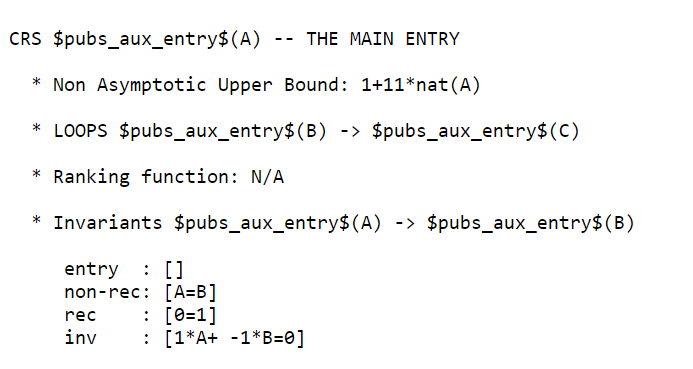
\includegraphics[width=0.9\textwidth]{pubs_example2.png}
    \caption{Esempio di output PUBS su Listing 6}
\end{figure}

\end{document}